\documentclass{report}
\usepackage[a4paper, margin=3cm]{geometry}
\usepackage[utf8]{inputenc}
\usepackage[ngerman]{babel}
\usepackage{todonotes}
\usepackage{amsmath}
\usepackage{amssymb}
\usepackage{amsfonts}
\usepackage{hyperref}
\usepackage{caption}
\usepackage{listings}
\usepackage{subcaption}
\usepackage{float}
\usepackage{siunitx}

%Necessary for sha letter
\DeclareFontFamily{U}{wncy}{}
\DeclareFontShape{U}{wncy}{m}{n}{<->wncyr10}{}
\DeclareSymbolFont{mcy}{U}{wncy}{m}{n}
\DeclareMathSymbol{\Sh}{\mathord}{mcy}{"58} 

% Change emph to boldface instead of cursive
\DeclareTextFontCommand{\emph}{\boldmath\bfseries}

% Inline Vectors: $\icol{a\\b}$, $\irow{a&b}$
\newcommand{\icol}[1]{% inline column vector
  \left(\begin{smallmatrix}#1\end{smallmatrix}\right)%
}

\newcommand{\irow}[1]{% inline row vector
  \begin{pmatrix}#1\end{pmatrix}%
}

\newcommand{\norm}[1]{\left\lVert#1\right\rVert}
\newcommand*\diff{\mathop{}\!\mathrm{d}}
\newcommand*\Diff[1]{\mathop{}\!\mathrm{d^#1}}

\title{Neuroinformatik Summary}
\author{
  Dominik Authaler\\
  \texttt{dominik.authaler@uni-ulm.de}
  \and
  Jonas Otto\\
  \texttt{jonas@jonasotto.com}
  \and
  Marco Deuscher\\
  \texttt{marco.deuscher@uni-ulm.de}
  \and
   Luca Krüger\\
  \texttt{luca.krueger@uni-ulm.de}
  \and
  Carolin Schindler\\
  \texttt{carolin.schindler@uni-ulm.de}
}
\date{July 2019}


\begin{document}

\maketitle

\tableofcontents
\listoftodos


\todo[inline]{Verbesserungen des überwachten Lernen (Quickprop etc.)}
\todo[inline]{Allgmein einfügen der Erkenntnisse aus den Übungsblätter}
\todo[inline]{}

\chapter{Neuronale Modelle}
\todo[inline]{ausführtlicher da anscheinend doch nicht ganz unwichtig für die klausur}
Es wird in vielen Modellen eine Schichtenstruktur übernommen, wie sie bspw. in der Großhirnrinde zu finden ist.\\
Neuron besteht aus Zellkörper, Dendriten und Axon. Nervenimpuls breitet sich vom Axonhügel über gesamtes Axon aus.\\
Synapsen sind die Kopplungen zwischen Neuronen.\\
Das Ruhepotential liegt bei ca. $-75\si{\milli \volt}$. Spikes haben Amplitude bis ca. $+30\si{\milli \volt}$. Danach leichtes Unterschwingen bis Ruhepotential wieder erreicht wird.\\
Am Neuron werden die Aktionspotentiale zeitlich und räumliche summiert/integriert. Wenn Schwellwert erreicht wird, feuert das Neuron.

\section{Neuronale Verarbeitung}
\begin{enumerate}
    \item NN bestehen aus Neuronen, welche über Synapsen verbunden sind
    \item Neuronen senden über Axon Aktionspotentiale aus
    \item Neuronen summieren/integrieren ankommende AP auf
    \item wird Schwellwert überschritten feuert Neuron\\
        wird Schwellwert nicht überschritten feuert Neuron nicht
\end{enumerate}

\section{Hodgkin-Huxley Modell}
\begin{itemize}
    \item es handelt sich hierbei um ein komplexes Neuronenmodell
    \item neurophysiologische Experimente an Zellmembran von Tintenfisch als Grundlage $\rightarrow$ Erkenntnisse zu Ruhepotential und Weiterleitung der AP
    \item Modell enthält Charakteristika der Ionen-Kanäle
\end{itemize}
$\rightarrow$ Auf Grund der hohen Komplexität nicht für große Netze geeignet


\subsection{Ersatzschaltbild der Axonmembran}
In \ref{ch_bio_esb} ist das ESB für die Axonmembran zu sehen. Es werden die Kalium-, Natrium-,Leck/Chloridströme modelliert. Die Membrankapazität wird durch einen Kondensator modelliert. Der Gesamtstrom ergibt sich als Summe der drei Teilströme 
\begin{equation*}
    I_{Ionen} = I_K + I_{Na} + I_L = G_K(U-E_K) + G_{Na}(U-E_{Na}) + G_L(U-E_L)
\end{equation*}
Das Membranpotential ist durch die DGL
\begin{equation*}
    C\frac{dU}{dt} = I_{ext}-I_{Ionen}
\end{equation*}
gegeben, wobei $I_{ext}$ ein externer Strom ist. Die oben verwendeten Größen selbst werden alle wieder erneut durch DGLn beschrieben.\\
$\rightarrow$ Es können keine analytischen Lösungen bestimmt werden.\\
Das Modell beschreibt das biologische Vorbild recht gut. (siehe Skript für genaue Ergebnisse)\\
In der Praxis ist das Modell zu komplex und rechenintensiv.


\begin{figure}[h]
    \centering
    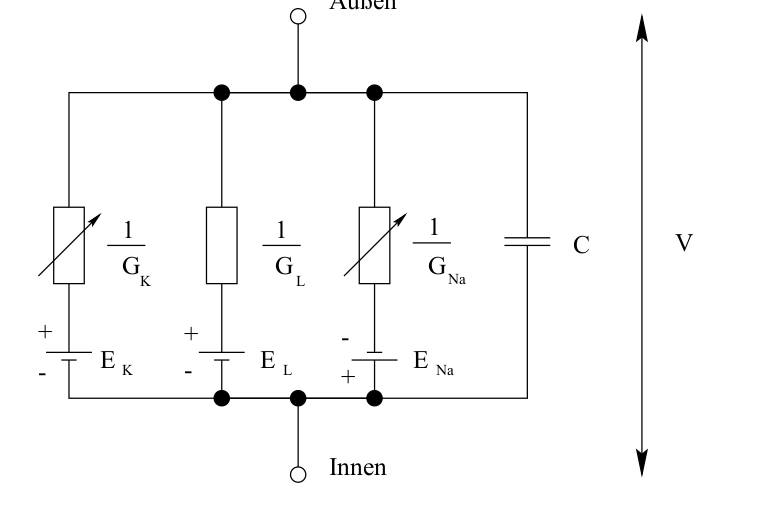
\includegraphics[width=0.75\textwidth]{img/BiologischesModell/ESB.png}
    \caption{Ersatzschaltbild für Axonmembran}
    \label{ch_bio_esb}
\end{figure}


\section{Kontinuierliches Modell}
\begin{itemize}
    \item keine Modellierung der einzelnen Ionen-Kanäle mehr
    \item Beschreibung eines Neurons durch zwei Gleichungen
        \begin{itemize}
            \item DGL dentritisches Membranpotential $u_j(t)$
            \item Axonales Membranpotential durch Funktionsauswertung $y_j(t)=f(u_j(t))$
        \end{itemize}
    \item synaptische Kopplungen werden durch reelle Zahlen $c_{ij}$ beschrieben.
    \item räumliche und zeitliche Integration: Summation der AP nach Gewichtung mit synaptischen Kopplungsstärken
\end{itemize}

\subsection{Modellgleichung}
\begin{align*}
    \tau \Dot{u}_j(t) & = -u_j(t) + x_j(t) + \sum_{i=1}^n c_{ij}y_i(t-d_{ij})\\
    y_j(t) &= f_j(u_j(t))
\end{align*}

Hierbei ist $\tau$ eine Zeitkonstante $>0$. $u_j(t)$ das dentritische Potential. $x_j(t)$ der externe Input. $c_{ij}$ die synaptische Kopplungsstärke. $d_{ij}$ die Laufzeit. $y_j(t)$ das axonale Potential und $f_j(x)$ die j-te Transferfunktion.\\

Auch diese DGL ist nicht analytische lösbar. Es kann aber eine Näherungslösung bestimmt werden durch diskretisieren der Zeit. Es ergibt sich dann

\begin{equation*}
    \Dot{u}_j(t) = \frac{u_j(t+\Delta t)-u_j(t)}{\Delta t}
\end{equation*}

daraus ergeben sich die 

\subsubsection{Diskrete Modellgleichungen}
\begin{align*}
    \frac{\tau}{\Delta t}(u_j(t+\Delta t)-u_j(t)) & = -u_j(t) + x_j(t) + \sum_{i=1}^n c_{ij}y_i(t-d_{ij})\\
    y_j(t) &= f(u_j(t))
\end{align*}

\subsection{Einfache Transferfunktionen}
\begin{itemize}
    \item Lin. Fkt $f(x) = x$ $\rightarrow$ lineares Neuron
    \item Heavisidefunktion $\rightarrow$ Schwellwertneuron
    \item Stückweise lineare Funktion $f (x) = \left\{
                                        \begin{array}{ll}
                                        0 & x \leq 0 \\
                                        x & \, x\in[0,1] \\
                                        1 & x\geq 1
                                        \end{array}
                                        \right. $
    \item logistische Funktion $f(x) = \frac{1}{1+\exp{-\beta x}}$                         
\end{itemize}

Die Funktionen (2)-(4) liegen im Wertebereich $[0,1]$. Es kann aber auch der Wertebereich $[-1,1]$ wünschenswert sein (dann bspw. mit Tanh).

\subsection{Neuronenmodell in Anwendungen}
\begin{figure}[h]
    \centering
    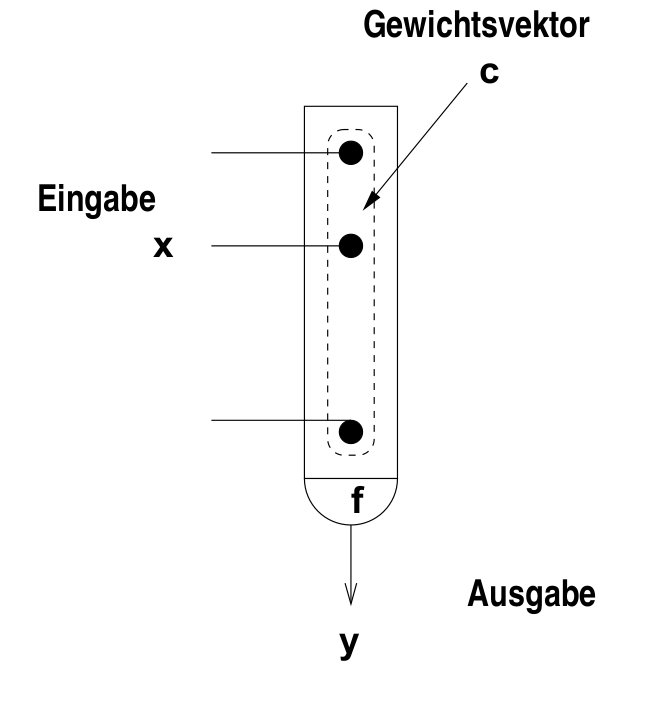
\includegraphics[width=0.25\textwidth]{img/BiologischesModell/NeuronenmodellAnwedung.png}
    \caption{Neuronenmodell in Anwedungen}
    \label{ch_bio_nmAnwendung}
\end{figure}

Für das Neuronenmodell in Anwendungen werden die folgenden Vereinfachungen gemacht
\begin{itemize}
    \item Neuronen ohne Gedächnis
    \item vernachlässigen der Signallaufzeit $d_{ij}$
\end{itemize}
Einige Beispiele

\paragraph{Lineares Neuron}
\begin{equation*}
    y(x) = \langle x,c \rangle + \Theta = \sum_{i=0}^n x_ic_i + \Theta
\end{equation*}

\paragraph{Schwellwert Neuron}
\begin{equation*}
    y (x) = \left\{
                                        \begin{array}{ll}
                                        1 & \,\langle x,c \rangle \geq \Theta \\
                                        0 & \, \text{sonst} \\
                                        \end{array}
                                        \right. 
\end{equation*}

\paragraph{Kontinuerliches nicht lineares Neuron}
\begin{equation*}
    y(x) = f(\langle x,c \rangle + \Theta)
\end{equation*}
wobei $f$ eine Transferfunktion.\\

Es muss aber nicht unbedingt immer das Skalarprodukt verwendet werden, andere Beispiele sind

\paragraph{Distanzberechnendes Neuron}
\begin{equation*}
    y(x) = \norm{x-c}_2
\end{equation*}

\paragraph{Radial symmetrisches Neuron}
\begin{equation*}
    y(x) = h(\norm{x-c}_2) \quad \text{mit } h(r) = \exp{-\frac{r^2}{2\sigma^2}}
\end{equation*}


\chapter{Neuronale Architekturen}

\section{Rückgekoppelte Netze}
Neuronen sind beliebig miteinander verbunden, d.h. jedes Neuron kann mit jedem anderen Neuron verbunden sein. Die Kopplungsmatrix C hat keine spezielle Struktur.
\begin{figure}[h]
    \centering
    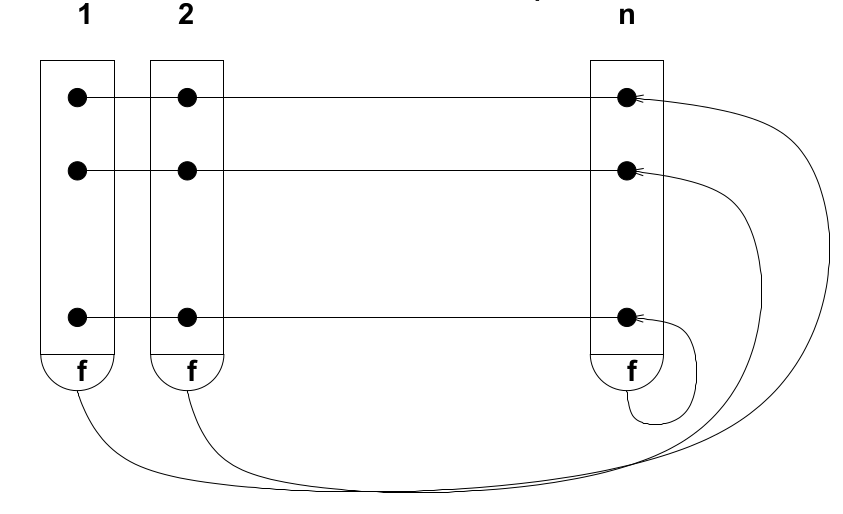
\includegraphics[width=0.25\textwidth]{img/NeuronaleArchitekturen/rueckgekoppelteNetze.png}
    \caption{Rückgekoppeltes Netz}
    \label{ch_arch_rueck}
\end{figure}

\section{Vorwärtsgekoppelte Netze}
\begin{itemize}
    \item Informationsfluss gerichtet: Eingabeneuron $\rightarrow$ Ausgabeneuron
    \item sequentielle Verarbeitung durch mehrere Neuronen/Schichten
    \item C ist durch eine Matrix gegeben $\rightarrow$ Graph zyklenfrei
\end{itemize}
Diese Art der Netze sind für die praktische Anwendung von großer Bedeutung.

\section{Geschichtete neuronale Netze}
\begin{itemize}
    \item Neuronen in Eingabeschicht geben Input nur weiter
    \item Neuronen in Schicht k: Input von k-1, Output an k+1 (hidden layer)
    \item letzte Schicht als Ausgabeschicht
\end{itemize}

\section{Darstellung von Mehrschicht-Netzen}
\begin{figure}[h]
    \centering
    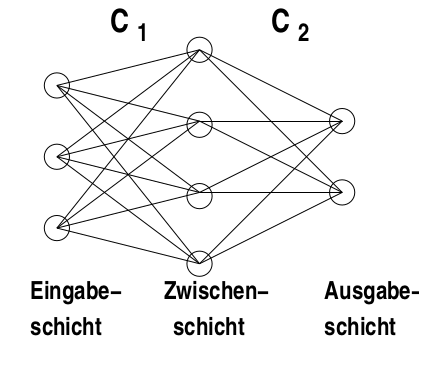
\includegraphics[width=.3\textwidth]{img/NeuronaleArchitekturen/d1.png}\hfill
    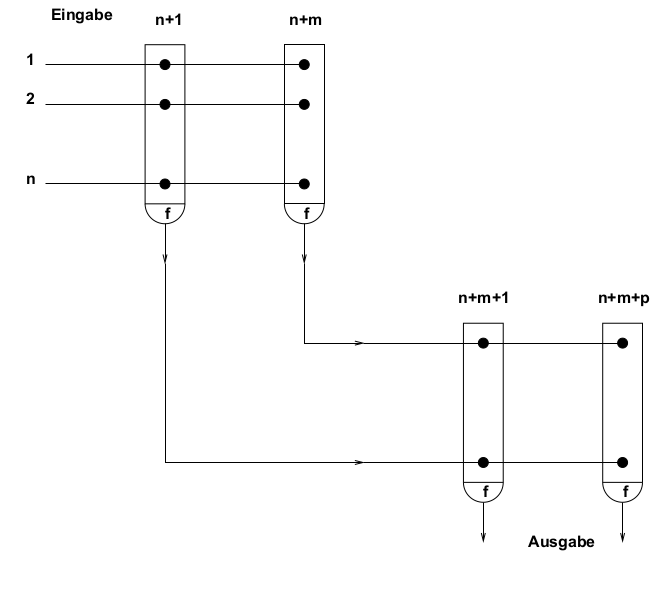
\includegraphics[width=.3\textwidth]{img/NeuronaleArchitekturen/d2.png}\hfill
    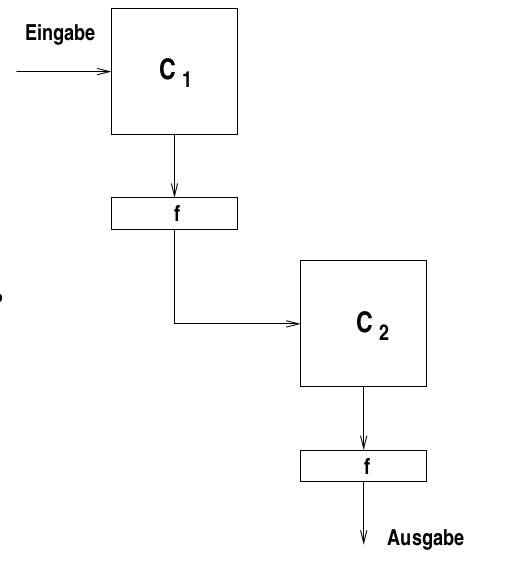
\includegraphics[width=.3\textwidth]{img/NeuronaleArchitekturen/d3.png}
    
    \caption{Darstellungsmöglichkeiten}
    \label{ch_arch_darst}
\end{figure}

\chapter{Lernregeln für neuronale Netze}
\emph{Lernen} als erwerb von Wissen. \emph{Gedächtnis} gelerntes Wissen kann wiedergefunden werden.\\
Es kann gelernt werden  durch verändern der Verbindungsstruktur (Anzahl Neuronen/ Schichten) oder Ändern der Verbindungsstärken. 

\section{Lernen durch Änderung der Synapsenstärke}
\begin{itemize}
    \item Änderung der Synapsenstärke durch DGL beschrieben
    \item Änderung der synaptischen Kopplungen deutlich langsamer als Änderung der neuronalen Zustände
\end{itemize}
$\rightarrow$ Praxis: Lernen von der Anwednungsphase getrennt

\paragraph{Aufwand beim Lernen in Netz mit n Neuronen}
Es sind $n^2$ Multiplikationen nötig um Zustände aller n Neuronen festzustellen. Bei einer DGL pro Synapse bereits $n^2$ DGLn\\
$\rightarrow$ Zu großer Aufwand. Skaliert nicht für große Netze.

\section{Allgemeine lokale Lerneregel}
Ändern einer synaptischen Kopplung $c_{ij}$ soll durch lokale Größen bestimmt sein. Diese Idee ist auch biologisch sinnvoll.
\paragraph{DGL}
\begin{equation*}
    \Delta c_{ij}(t) = c_{ij}(t) - c_{ij}(t-\Delta t) = -v(t)c_{ij}(t)+l(t)(y_i(t)-ac_{ij}(t)-b)(\delta_i(t)-c)
\end{equation*}
Meist wird $\Delta t=1$ gewählt. $v(t)$ ist die Vergessensrate, häufig $v(t) = 0$. $l(t)$ ist die Lernrate, i.d.R. $l(t)>0$ monoton fallend. $a,b,c$ Konstanten, meist $a=b=c=0$. $\delta_i(t)$ Form wird durch Art des Lernens bestimmt.

\subsection{Unüberwachtes Lernen (Hebb'sche Lernregel)}
Wähle $\delta_j(t) = u_j(t)$ oder $\delta_j(t) = y_j(t)$\\
\begin{equation*}
    \Delta c_{ij}(t) = l(t)y_i(t)y_j(t) \qquad \text{(Hebb'sche Lernregel)}
\end{equation*}
\textbf{Idee:} \textit{Wenn Axon der Zelle A nahe genug ist, um eine Zelle B zu erregen, kommt es zu einem Wachstumsprozess in einer oder beiden Zellen. Die Effizienz von Zella A auf Zelle B wächst}

\section{Überwachtes Lernen}
\begin{itemize}
    \item Es ist ein Lehrersignal $T_j$ des j-ten Neurons gegeben
    \item Ausgabe $y_i$ beeinflusst $y_j$ über $c_{ij}$
\end{itemize}
\textbf{Idee:} Ausgabe $y_j$ soll durch Änderung der synaptischen Kopplungsstärke $c_{ij}$ möglichst auf das Lehrersignal $T_j$ geregelt werden.

\subsection{Delta-Lernregel}
$\delta_j$ hat die Form $d_j(t) = T_j - y_j(t)$, also
\begin{equation*}
    \Delta c_{ij}(t) = l(t)y_i(t)(T_j(t)-y_j(t))
\end{equation*}

\subsubsection{Delta-Lernregel für nicht lineares Neuron}
$y_j(x) = f(\sum_{i=1}^nc_{ij}y_i)$ und $u_j = \sum_{i=1}^nc_{ij}y_i$ und $f$ ist eine diff'bare Transferfunktion.\\
Für die Änderung der Ausgabe ergibt sich dann
\begin{align*}
    y_j^{neu} -y_j & =  f(\sum_{i=1}^nc_{ij}^{neu}y_i) - f(\sum_{i=1}^nc_{ij}y_i)\\
    &= f'(z)(u_j^{neu}-u_j)\\
    &= f'(z)(c_{ij}^{neu}-c_{ij})y_i\\
    &= lf'(z)(T_j-y_j)y_i^2\\
    &\rightarrow y_j^{neu} = y_j +  lf'(z)(T_j-y_j)y_i^2
\end{align*}

Man kann hier leicht sehen, dass wenn $T_j = y_j$ bereits gegeben ist keine Veränderungen mehr stattfinden. Ansonsten ändert sich der Output in Richtung des Lerhersignals.\\
Ist die Lernrate $l>0$ wird der Fehler kleiner.

\subsection{Kostruktion von Lernregeln}
\textbf{Ziel:} Lernverfahren soll Fehler zw. Lehrer und Netzausgabe minimieren\\
Es sind Trainingsdaten gegeben durch
\begin{equation*}
    T = \{(x^\mu,T^\mu) \quad|\quad x^\mu \in \mathbb{R}^d, T^\mu \in \mathbb{R}^n, \mu=1,\dots,M\}
\end{equation*}

Der Unterschied vom Lehrer zur Ausgabe wird durch eine Abstandsfunktion gemessen

\begin{equation*}
    \norm{T^\mu - y^\mu}_p = (\sum_{i=1}^n (T^\mu - y^\mu)^p)^{\frac{1}{p}}
\end{equation*}
mit p=1 ergibt sich der Manhatten Abstand und für p=2 die euklidische Norm.\\
Die Netzausgabe $y$ hängt von der Kopplungsmatrix $C$ ab ($y=y(C)$).\\
$\rightarrow$ es wird $C^*$ gesucht, so dass Fehler minimal.\\
Definiere Fehler $E(C) = \sum_{\mu=1}^M \sum_{j=1}^n(T_j^\mu - y_j^\mu)^2$

\subsection{Optimieren der Zielfunktion}
Die Fehlerfunktion ist eine reelle Funktion: $E(C): \mathbb{R}^r\to \mathbb{R}$. Es wird ein $C^*$ gesucht, so dass die Fehlerfunktion E minimiert wird. 
\begin{equation*}
    E(C^*)\leq E(C) \quad \forall C
\end{equation*}
Dann ist $C^*$ ein globales Minimum, in der Regel nicht analytisch berechenbar.\\
Es werden numerische Methoden zum finden eines lokalen Minimums verwendet.\\
\textbf{Verfahren:}
\begin{enumerate}
    \item $t=0$, Wähle $l>0$ und Startwert $C(0)$ und $\epsilon>0$
    \item Iterierte Vorschrift $t=0,1,\dots,\text{bis }\norm{\Delta C}<\epsilon$
\end{enumerate}

\subsection{Lernregeln für einschleifige Netze}
Trainingsmenge $ T = \{(x^\mu,T^\mu) \quad|\quad x^\mu \in \mathbb{R}^d, T^\mu \in \mathbb{R}^n, \mu=1,\dots,M\}$\\
Das Neuronale Netz besteht aus einer Schicht (ohne Inputlayer) aus n nicht linearen Neuronen

\paragraph{Vorwärtsphase}
\begin{enumerate}
    \item $u_j^\mu = \langle x,c_j\rangle$
    \item Netzausgabe $y_j^\mu = f(u_j^\mu)$
\end{enumerate}

\paragraph{Gradientenverfahren}
Definiere Fehlerfunktion zu $E(C) = \sum_{\mu=1}^M\norm{T^\mu-y^\mu}_2^2\rightarrow \text{min}$

\begin{enumerate}
    \item $\frac{\partial}{\partial c_{ij}}E(C) = \sum_{\mu=1}^M 2(T_j^\mu-y_j^\mu)(-f'(u_j^\mu))x_i^\mu$
    \item $c_{ij}(t+1) = c_{ij}(t) + l(t)\sum_{\mu=1}^M 2(T_j^\mu-y_j^\mu)(-f'(u_j^\mu))x_i^\mu$
\end{enumerate}
Dies entspricht der Batch-Lernregel, da alle Trainingsdaten dem Netz präsentiert werden, bevor die Gewichte angepasst werden.

\paragraph{Inkrementelle Version}
\begin{equation*}
    c_{ij}(t+1) = c_{ij}(t)+2l(t)(T_j^\mu-y_j^\mu)x_i^\mu
\end{equation*}

Dieses Verfahren wird so lange iteriert bis der Fehler kleiner als eine zuvor festgelegte Güte ist.

\subsection{Lernen beim Perzeptron}
Grundidee des Perzeptrons als Schwellwertneuron:\\
Dendritisches Potential:
\begin{equation*}
    u=\sum_{i=1}^m x_i w_i + b
\end{equation*}
Ausgabe:
\begin{equation*}
    y= \begin{cases}
        1 &\text{für } u \geq 0\\
        0 &\text{sonst}
    \end{cases}
\end{equation*}
So ein Perzeptron kann Daten in 2 Klassen separieren, im zweidimensionalen Fall z.B. durch eine Gerade.
\paragraph{Lernalgorithmus}
Für jedes Muster (Eingabe $x$ mit Lehrersignal $T$ wird dieser Lernschritt durchgeführt:
\begin{enumerate}
    \item Berechnen der Ausgabe $y$ des Netzes aufgrund der Eingabe $x$
    \item Berechnen des Fehlers $\delta = T - y$ mit Lehrersignal $T$
    \item Anpassen der Gewichte $w_i(t+1) = w_i(t) + \eta \delta x_i$
\end{enumerate}
Der Bias $b$ kann als weiteres Gewicht mit konstantem Eingang betrachtet werden und muss beim Lernen nicht explizit betrachtet werden.\\
Falls eine Lösung existiert ($\iff$ Klassen sind linear separierbar) konvergiert dieser Lernalgorithmus in endlicher Zeit
(Beweis Seite 90f).
\todo[inline]{Beweis aufschreiben oder für irrelevant erklären}

\subsection{Lernen beim Multi Layer Perzeptron (MLP)}
Hier werden nicht nur mehrere Perzeptrons(?) verwendet, die Neuronen haben beim MLP auch eine sigmoide Funktion
(z.B. $f(x) = \frac{1}{1+\exp{(-\beta x)}}$) als Transferfunktion (notwendig für Differenzierbarkeit).
\todo[inline]{Ist das noch ein Perzeptron wenn man andere Fehlerfunktion verwendet?}
Für die Fehlerfunktion $E(T)$ wird hier die quadratische Fehlerfunktion $E(T)=|T-y|^2=\sum_{i=1}^m (T_i-y_i)^2$ verwendet.
Der gesamte Fehler über alle Muster berechnet sich aus der Summe über die Fehler jedes einzelnen Musters.
(Einsetzen der Formel mit Absicht weggelassen weil Indexschlacht)\\
Das Lernen erfolgt hier wieder per Gradientenabstieg, um ein (lokales) Minimum der Fehlerfunktion zu finden.
Für das Lernen von Gewichten muss aufgrund der vielen Layer \emph{Backpropagation} verwendet werden:

\paragraph{Backpropagation (Online)}
Das Prinzip bei Backpropagation ist es, die Fehler, die initial nur von der letzten (Ausgabe-)Schicht ablesbar sind, von hinten nach vorne zu propagieren, um in jeder Schicht Gewichte anzupassen. Dies wird für alle Trainingsdaten ausgeführt, was dann eine \emph{Epoche} genannt wird.\\
Algorithmus für eine Epoche:\\
\todo[inline]{Für mehr Lesbarkeit Indices durch Beschränkung auf einzelne Neuronen eliminieren}
Für jedes Muster $x$ mit Lehrersignal $T$:
\begin{enumerate}
    \item Vorwärtsphase: Berechnen der Netzwerkausgabe $y$ für ein Muster $x$
    \item Fehlerberechnung für alle Ausgabeneuronen $j=1\dots n$ anhand des Lehrersignals $T$:\\
        $\delta_j^{(n)} = (T_j - y_j)f'(u_j^{(n)})$
    \item Fehlerrückvermittlung (Schicht $k = 1\dots n-1$ mit $i$ Neuronen, $j$ Neuronen in nachfolgender Schicht $k+1$):\\
        $\delta_i^{(k)} = \sum_j w_{ij}^{(k+1)} \delta_j^{(k+1)} f'(u_i^{(k+1)})$\\
        (Hierbei iteratives Vorgehen von $k=n-1$ bis $k=1$)
    \item Lernen: In Schicht $k$ für jedes Gewicht der Eingabe $i$ auf Neuron $j$: $w_{ij} = w_{ij} + \eta y_i^{(k-1)} \delta_j$,
        dabei ist $y_i^{(k-1)}$ die Ausgabe der vorherigen Schicht bzw beim ersten Layer die Eingabe in das Netzwerk $x$.
\end{enumerate}
Obwohl in jeder Epoche jedes Muster benutzt wird, ist das Lernen erst nach mehreren Epochen abgeschlossen.

\paragraph{Backpropagation (Batch)}
Auch bei Backpropagation können die Trainingsdaten zu Batches zusammengefasst werden.\\
Ein Gewichtsupdate findet hier erst nach Präsentation aller Muster des Batches statt, der Lernschritt
lautet nun $w_{ij} = w_{ij} + \eta \sum_\mu y_{\mu i}^{(k-1)} \delta_{\mu j}$.
\todo[inline]{Batch Modus überprüfen}

\todo[inline]{Backprop. mit Momentum}



\section{Unüberwachtes Lernen}

\subsection{Neuronale Merkmalskarten}
Übernehme Idee der Lokalität aus dem biologisches Vorbild. (siehe Skript Folie 145ff. für genaue Beschreibung)

\paragraph{Problem}
Man hat sehr viele Datenpunkte in einem hochdimensionalen Merkmalsraum. Außerdem sind häufig zu Beginn der Analyse noch nicht alle Datenpunkte bekannt. Vor allem sind \textbf{keine} Lehrersignale vorhanden.

\subsection{Reduktion der Datenpunkte}
\paragraph{Ziele}
\begin{itemize}
    \item Repräsentation der Eingabedaten bestimmen
    \item prototypische Repräsentationen sollen berechnet werden 
    \item Ähnliche Daten werden durch gleichen Prototyp repräsentiert
    \item Regionen mit hoher Datendichte sollen durch mehrere Prototypen repräsentiert werden
    \item erstellen einer Kartenstruktur, benachbarte Neuronen/Prototypen sollen durch ähnliche Eingaben aktiviert werden
\end{itemize}

\subsection{Kompetetives neuronales Netz}

\begin{figure}[h]
    \centering
    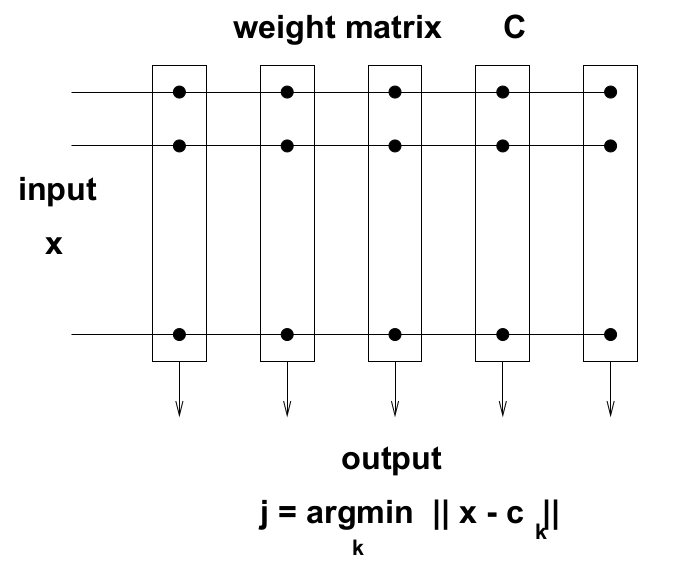
\includegraphics[width=.33\textwidth]{img/NeuroLernregel/kompNetz.png}
    \caption{Architektur komp. Netz}
    \label{ch_lern_upstart}
\end{figure}

\subsubsection{Distanz vs. Skalarprodukt zur Gewinnerdetektion}
Die euklidische Norm ist gegeben durch
\begin{equation*}
    \norm{x}_2 = \sqrt{\langle x,x \rangle}
\end{equation*}
Damit gilt für den Abstand von $x,y\in\mathbb{R}^n$
\begin{equation*}
    \norm{x-y}_2^2 = \langle x-y,x-y \rangle = \langle x,x\rangle -2\langle x,y\rangle + \langle y,y\rangle = \norm{x}_2^2 - 2\langle x,y \rangle + \norm{y}_2^2
\end{equation*}
Dann gilt für die Gewinnerdetektion bei der Eingabe $x$ unter den durch $c_1,\dots,c_k$ und $\norm{c_i}_2=1$ gegebenen Neuronen 
\begin{equation*}
    j^* = \operatorname{argmax}_i \langle x,c_i \rangle \quad \Longleftrightarrow \quad j^* = \operatorname{argmin}_i \norm{x-c_i}_2
\end{equation*}

\subsection{Kohonen's selbstorganisierende Karte}
\begin{figure}[h]
    \centering
    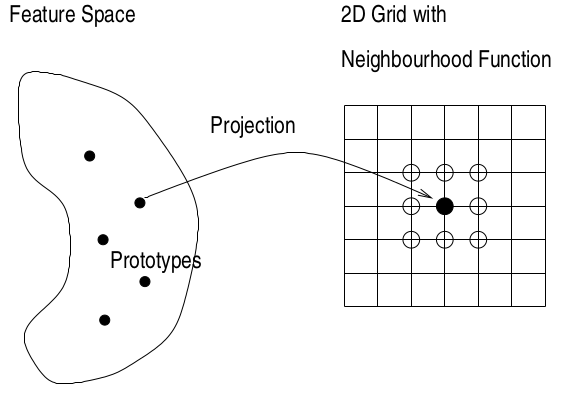
\includegraphics[width=.33\textwidth]{img/NeuroLernregel/SOM.png}
    \caption{Darstellung der Kohonen Karte}
    \label{ch_lern_SOM}
\end{figure}
\paragraph{Ziele}
\begin{itemize}
    \item Berechnung von Prototypen im Merkmalsraum, also $c_i \in \mathbb{R}^d$, die die gegebenen Daten $x\in\mathbb{R}^d$ gut repräsentieren
    \item Nachbarschaftserhaltende Abbildung der Prototypen $c_i\in\mathbb{R}^d$ auf Gitterpositionen $g$ auf ein Gitter im $\mathbb{R}^2$
\end{itemize}

Es kann damit die Kohonen Lernregel formuliert werden
\begin{equation*}
    \Delta c_{ij} = l_t N_t(g_j,g_{j^*})\cdot(x-c_j)
\end{equation*}

Hierbei ist $j^*$ der Gewinner, $N_t$ eine Nachbarschaftsfunktion, $g_j$ die Gitterposition des j-ten Neurons auf der Karte und $l_t$ und $\sigma_t$ sind trainingszeitabhängige Lernraten bzw. Nachbarschaftsweitenparameter. Diese beiden Parameter sollten bei steigender Trainingszeit t gegen $0$ konvergieren.\\
Eine mögliche Nachbarschaftsfunktion ist gegeben durch $N_t(g_j,g_{j^*} = \exp{(-\frac{\norm{g_j-g_{j^*}}_2^2}{2\sigma_t^2})}$

\subsection{Kohonen Lernalgorithmus}
Gegeben ist der Input $X = \{x_1,\dots,x_M\}\subset \mathbb{R}^d$

\begin{enumerate}
        \item Wähle $r,s\in\mathbb{N}$ eine Clusterzahl $k=rs\in\mathbb{N}$, eine Lernrate $l_t>0$ und eine Nachbarschaftsfunktion $N$ und maximale Lernepochenzahl $N_{max}$. $t=0$
        \item Initialisiere die Prototypen $c_1,\dots,c_k \in\mathbb{R}^d$, diese bilden Matrix $C\in\mathbb{R}^{k\times d}$
        \item Jeder Prototyp auf genau eine Gitterposition $g_i \in \{1,\dots,r\}\times\{1,\dots,2\}$
        \item \texttt{\textbf{repeat}\\
            Wähle $x\in X$ und $t=t+1$\\
            $j^* = \operatorname{argmin}_i\norm{x-c_i}$ (winner detection)\\
            \textbf{for all j:}\\
            $c_j = c_j + l_tN_t(g_j,g_{j^*}(x-c_j)$ (update)}
        \item bis $t\geq N_{max}$    
\end{enumerate}
Siehe Skript Folie 161 ff. für Anwendungsbeispiel.


\subsection{Kompetetives Lernen}
Gegeben ist der Input $X = \{x_1,\dots,x_M\}\subset \mathbb{R}^d$
\begin{enumerate}
    \item Wähle Clusterzahl $k\in\mathbb{N}$ und eine Lernrate $l_t>0$ und $N$. $t=0$
    \item Initialisiere Prototypen $c_1,\dots,c_k\in\mathbb{R}^d$ bilden dann Matrix $C\in\mathbb{R}^{k\times d}$
    \item \texttt{\textbf{repeat}\\
        Wähle $x\in X$ und $t=t+1$\\
        $j^* = \operatorname{argmin}_i\norm{x-c_i}_2$ (winner detection)\\
        $c_{j^*} = c_{j^*} + l_t(x-c_{j^*})$ (winner update)}
    \item bis $t\geq N$
\end{enumerate}

\todo[inline]{einfügen der Notizen aus der Vorlesung}

\subsection{k-means Clusteranalyse}
Der Datenpunkt $x\in\mathbb{R}^d$ wird dem nächsten Clusterzentrum $c_{j^*}$ zugeordnet.
\begin{equation*}
    j^* = \operatorname{argmin}_j\norm{x-c_j}
\end{equation*}
Das Clusterzentrum wird dann angepasst
\begin{equation*}
    \Delta c_{j^*} = \frac{1}{|C_{j^*}|+1}(x-c_{j^*})
\end{equation*}
Vergleich zum kompetitiven lernen
\begin{equation*}
    \Delta c_{j^*} = l_t(x-c_{j^*})
\end{equation*}


\subsection{ART-Netzwerke (Adaptive-Resonanz-Theorie}
Im folgenden wird nur die Grundlegende ART1 Architektur. Auf dieser aufbauend gibt es verschiedene Erweiterungen ART2, ART3, FuzzyART und ARTMAP.\\
Bei ART-Netzen handelt es sich um kompetitive Netze. ART-Netze sind wachsende Netze. Die maximale Anzhal der Neuronen ist jedoch beschränkt.\\
Bei ART1-Netzen sind die Eingabedaten und die Gewichtsvektoren/Prototypen binäre Vektoren.

\subsubsection{ART1-Lernen}
\begin{itemize}
    \item Inputvektoren und Prototypen $\in\{0,1\}^d$
    \item es wird nur der Gewichtsvektor des Gewinnerneurons $c_{j^*}$ adaptiert
    \item ist Ähnlichkeit zwischen Input $x$ und Prototyp $c_{j^*}$ zu gering, so wird durch $x$ ein neuer Prototyp definiert und $c_{j^*}$ wird nicht verändert
    \item Ähnlichkeit wird durch Skalarprodukt $\langle x,c_j \rangle$ gemessen
    \item Schranke für Mindestähnlichkeit wird durch Vigilanzparameter bestimmt
    \item ist Ähnlichkeit größer als Schranke, so wird $c_{j^*}$ durch komponentenweises \textbf{AND} von $x$ und $c_{j^*}$ adaptiert
    \item maximale Anzahl an Neuronen wird vorgegeben
\end{itemize}

\paragraph{ART1-Algorithmus}
Der Eingabevektor $x_\mu \in \{ 0,1 \}^d$ mit $\mu=1,\dots,M$, die Gewichtsvektoren bzw. Prototypen sind gegeben durch $c_i\in \{ 0,1 \}^d$. Mit $\textbf{1} = (1,1,\dots,1)\in \{ 0,1 \}^d$ wird der Eins-Vektor bezeichnet. $k$ ist die Anzahl der maximal möglichen Neuronen. Durch $\norm{x}_1$ ist die Eins-Norm definiert, diese gibt die Anzahl der Einsen an. Durch $\rho\in[0,1]$ ist der Vigilanzparameter gegeben.\\

\begin{enumerate}
    \item \texttt{Wähle $k\in\mathbb{N}$ und $\rho\in[0,1]$}
    \item \texttt{Setze $c_i=\textbf{1}$ für alle $i=1,\dots,k$}
    \item \texttt{WHILE noch ein Muster $x$ vorhanden DO\\
        Lies $x$ und setze $I=\{1,\dots,k\}$\\
        REPEAT\\
        $j^* = \operatorname{argmax}_{j\in I}\frac{\langle x,c_j\rangle}{\norm{c_j}_1}$ (winner detection)\\
        $I = I \setminus {j^*}$\\
        UNTIL $I=\emptyset$ or $\langle x, c_{j^*} \rangle \geq \rho \norm{x}_1$\\
        IF $\langle x, c_{j^*} \rangle \geq \rho \norm{x}_1$\\
        THEN $c_{j^*} = x\wedge c_{j^*}$ (winner update)\\
        ELSE keine Bearbeitung von $x$
        }
    \item \texttt{END}
\end{enumerate}
Zunächst werden die Hyperparameter $k$ und $\rho$ gewählt. Es werden dann die Gewichtsvektoren zu $\textbf{1}$ initialisiert. Es wird dann der Prototyp mit der größten Ähnlichkeit zu $x$ gesucht und der jeweilige Prototyp dann aus der Menge entfernt. Ist die Ähnlichkeit höher als der Schwellwert $\rho \norm{x}_1$ wird der Prototyp angepasst. Ist dies nicht der Fall tritt der Fall der Leerenmenge ein und $x$ wird implizit zu einem neuen Prototypen.

\subsection{LVQ (Lernende Vektorquantisierung)}
Bei LVQ handelt es sich um überwachte Lernverfahren zur Musterklassifikation. Bei LVQ-Verfahren handelt es sich um heuristische kompetitive Lernverfahren.\\
Es wird die euklidische Distanz zur Berechnung der Ähnlichkeit verwendet. Im folgenden wird nur LVQ1 behandelt. Es gibt diverese Erweiterungen wie LVQ2, LVQ3 und OLVQ.

\subsubsection{LVQ1-Algorithmus}
Der Input ist gegeben durch $X = \{(x_1,y_1),\dots,(x_M,y_M)\}\subset\mathbb{R}^d\times\Omega$ dabei ist $\Omega=\{1,\dots,L\}$ eine endliche Menge von Klassen(-Labels).

\begin{enumerate}
    \item \texttt{Wähle Prototypenzahl $k$, eine Lernrate $l_t>0$ und N. Setze $t=0$
    \item \texttt{Initialisiere Prototypen $c_1,\dots,c_k\in\mathbb{R}^d$}}
    \item \texttt{Bestimme für jeden Prototypen $c_i$ die Klasse $\omega_i\in\Omega$}
    \item \texttt{REPEAT\\
        Wähle ein Paar $(x,y)\in X$ und setze $t=t+1$\\
        $j^*=\operatorname{argmin}_i \norm{x-c_i}$ (winner detection + class from nearest neighbor\\
        IF $\omega_{j^*} \neq y$ THEN $\Delta = -1$ ELSE $\Delta = 1$ (check if classification result is correct)\\
        $c_{j^*} = c_{j^*} = l_t\Delta(x-c_{j^*})$ (winner update)}
    \item UNTIL $t\geq N$    
    
\end{enumerate}


\section{Konstruktive Lernverfahren}
Bei allen bisher behandelten Verfahren wird die Architektur des Netzes a priori festgelegt. Während des Trainings wird die Architektur also nicht mehr an das Problem angepasst.\\
Die Idee konstruktiver Lernverfahren ist es, mit einem kleinen Netz zu starten und während des Trainings bei Bedarf weitere Neuronen oder Schichten hinzuzufügen.

\subsection{Upstart-Algorithmus}
Der Upstart Algorithmus konstruiert Binärbäume aus Perzeptronen. Es handelt sich um einen rekursiven Algorithmus zum Erlernen beliebiger binärer Abbildungen mit Schwellwertneuronen.\\

\begin{figure}[h]
    \centering
    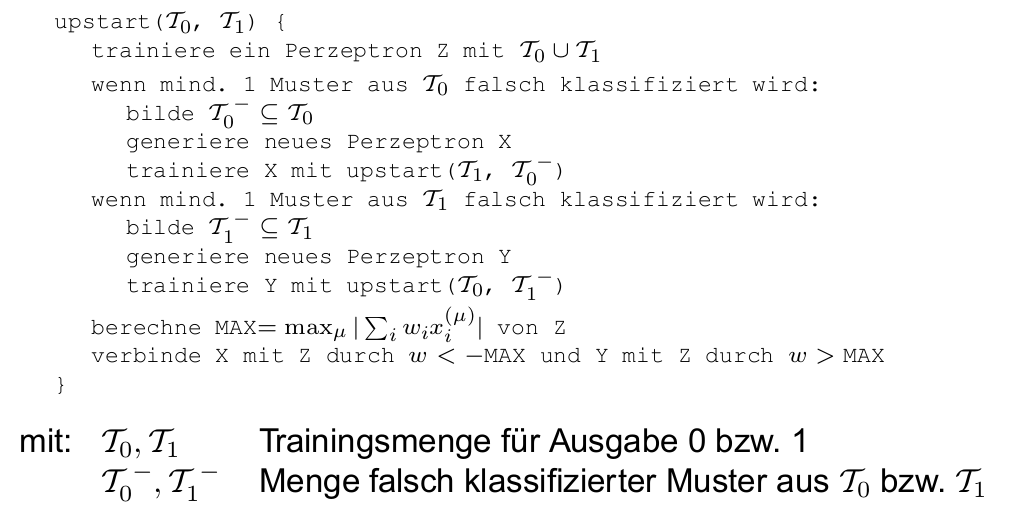
\includegraphics[width=1\textwidth]{img/NeuroLernregel/upstart.png}
    \caption{Upstart Algorithmus}
    \label{ch_lern_upstart}
\end{figure}

\subsection{Cascade Correlation}
\textbf{Motivation}: Bei einem großen Fehler am Ausgang für ein Muster werden alle Gewichte adaptiert. Da es keine Absprache zwischen den Neuronen gibt, kann es vorkommen, dass der Fehler für ein anderes Muster steigt. (\textit{moving target problem}).\\
\textbf{Idee}: Die Gewichte $v_{ij}$ eines verdeckten Neurons $j$ werden separat trainiert, indem die Korrlation zwischen Ausgabe des Neurons und dem Fehler maximiert wird. Danach werden die Gewichte $v_{ij}$ von Neuron $j$ eingefroren, es werden dann weitere verdeckte Neuronen hinzufügt, solange bis der Fehler am Ausgang ausreichend klein ist. 

\begin{figure}[h]
    \centering
    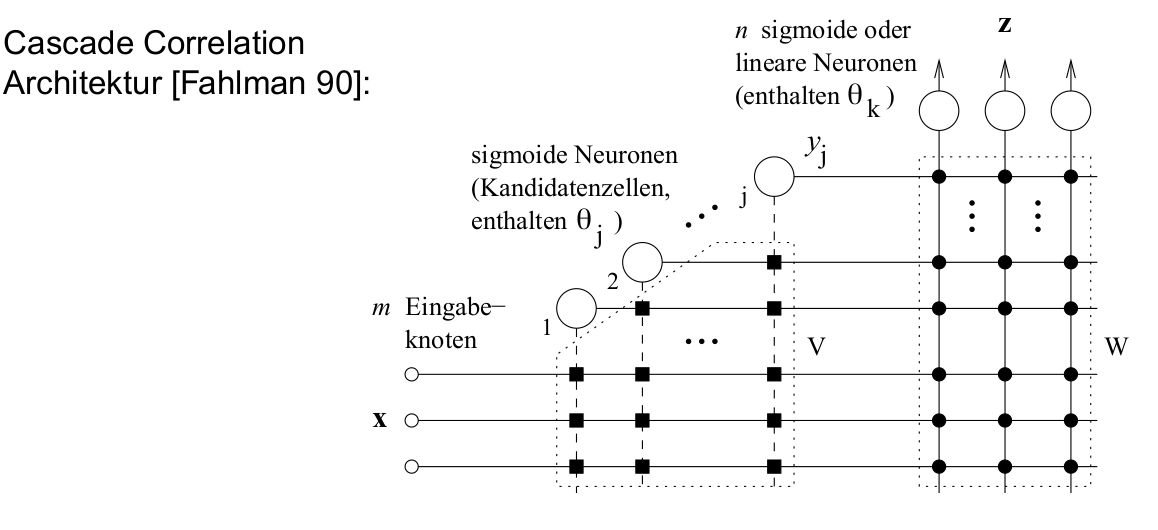
\includegraphics[width=.75\textwidth]{img/NeuroLernregel/cascade_corr_arch.png}
    \caption{Cascade Correlation Architektur}
    \label{ch_lern_cca}
\end{figure}

\todo[inline]{Herleitung der Lernregel (Folie 140/141}

\subsection{Zusammenfassung: Lernalgorithmus für Casecade Correlation}
\paragraph{Schritt (1):}
Trainiere die Gewichte $w_{ik}$ und $\Theta_k$ der Ausgangsknoten mit geeignetem Algorithmus
\begin{itemize}
    \item Perzeptron-Lernalgorithmus
    \item Delta-Lernregel
    \item Quickprop-Verfahren
\end{itemize}
solange bis der Fehler am Netzausgang nicht weiter sinkt.

\paragraph{Schritt (2):}
\begin{itemize}
    \item Stop, falls der Fehler $E$ bereits klein genug ist, sonst
    \item füge ein neues Neuron $j$ hinzu und initialisiere die Gewichte $v_{ij}$ zufällig
\end{itemize}

\paragraph{Schritt (3):}
Bestimme Gewichte  $v_{ij}$ und $\Theta_j$ des neuen Neurons $j$ derart, dass die Korrelation $S_j$ maximiert wird. Adaptiere hierfür $v_{ij}$ und $\Theta_j$ durch Gradientenaufstiegsverfahren, bis Korrelation $S_j$ nicht weiter steigt
\todo[inline]{ausführlicher}

\paragraph{Schritt (4):}
Friere alle Gewichte $v_{ij}$ und $\Theta_j$ des neuen Neurons ein.

\paragraph{Schritt (5):}
Gehe zu Schritt (1)


\chapter{Radiale Basisfunktionen (RBF)}
\section{Motivation für die Nutzung von RBF}
Es ist eine Lösung für das folgende Interpolationsproblem gesucht:\\
Es ist eine Menge von Trainingsdaten gegeben durch
\begin{equation*}
    M = \{(x^\mu,T^\mu) \quad | \quad x^\mu \in \mathbb{R}^m, T^\mu \in \mathbb{R}^n,\mu=1,\dots,p\}
\end{equation*}

\noindent Gesucht ist eine Funktion $g$, so dass gilt
\begin{equation*}
    %Was ist die undefined control sequence?!
    g: \mathbb{R}^m \to \mathbb{R}^n \quad \text{mit }g(x^\mu) = T^\mu \quad \forall \mu=1,\dots,p
\end{equation*}
\noindent Die Idee ist nun $g$ durch eine Linearkombination von p Funktionen $h_\nu(x) = h(\norm{x^\nu - x})$ mit belieb oft diff'barer radial symm. Funktion $h: \mathbb{R}^+ \to \mathbb{R}^+$\\
Das Interpolation wird also für $n=1$ bspw. durch
\begin{equation*}
    g(x^\mu)=\sum_{\nu=1}^p w_\nu h(\norm{x^\nu-x^\mu})=T^\mu \quad \forall \mu=1,\dots,p
\end{equation*}
gelöst. Die $w_\nu$ können analytischt bestimmt werden (siehe Skript Folie 125).

\subsection{Beispiele für radialsymm. Basisfunktionen}
Einige Beispiele für radialsymmetrische Basisfunktionen ($r=\norm{x-x^\mu})$
\begin{itemize}
    \item Gauss Funktion: $h(r) = \exp{(-\frac{r^2}{2\sigma^2})}$
    \item Inverse multiquadratische Funktion: $h(r) = \frac{1}{(r^2+c^2)^\alpha}$ mit $c\neq 0$ und $\alpha>0$
    \item Multiquadratische Funktion: $h(r) = (r^2+c^2)^\beta$ mit $c\neq0$ und $0<\beta\leq1$
\end{itemize}

\section{Aufbau eines RBF-Netzwerkes}
Im folgenden wird ein RBF Netzwerk beschrieben mit
\begin{itemize}
    \item $m$ Eingabeknoten
    \item $h$ RBF-Neuronen
    \item $n$ lineare Neuronen
\end{itemize}
Der Aufbau des Netzes ist in Abbildung \ref{ch_RBF_netz} zu sehen.

\begin{figure}[h]
    \centering
    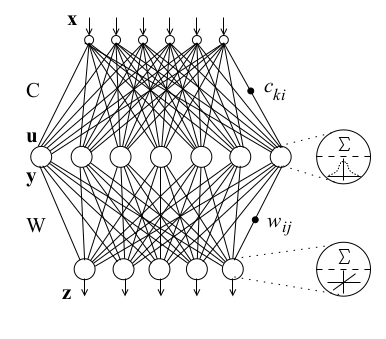
\includegraphics[width=0.4\textwidth]{img/RBF/RBFAufbau.png}
    \caption{RBF-Netzwerk}
    \label{ch_RBF_netz}
\end{figure}

Die Netzausgabe $z$ kann folgendermaßen berechent werden
\begin{align*}
    u_i &= \sqrt{\sum_{k=1}^m(x_k-c_{ki})^2} = \norm{x-c_i}\\
    y_i &= h(u_i)\\
    z_j &= \sum_{i=1}^h w_{ij}y_i [+\text{bias}_j]
\end{align*}

\section{Lernregel für RBF-Netzwerke}
Es wird nun eine Gradientenabstiegsverfahren für RBF-Netze hergeleitet
\begin{align*}
    \frac{\partial E}{\partial w_{ij}} &= \frac{\partial}{\partial w_{ij}}\norm{T-z}_2^2\\
    &= \frac{\partial}{\partial w_{ij}} \sum_j(T_j-z_j)^2\\
    &= -2(T_j-z_j)\frac{\partial}{\partial w_{ij}}\sum_i y_iw_{ij}\\
    &= -2y_i\delta_i
\end{align*}
Damit ergeben sich die folgenden Lernregeln\\
\paragraph{Online Modus}
\begin{align*}
    w_{ij}^{neu} &= w_{ij} - \eta_1 \frac{\partial E}{\partial w_{ij}} = w_{ij} + \eta_1 y_i\delta_j\\
    \text{bias}_j^{neu} &= \text{bias}_j - \eta_1 \frac{\partial E}{\partial w_{ij}}=\text{bias}_j +\eta_1\delta_j
\end{align*}

\paragraph{Batch Modus}

\begin{align*}
    w_{ij}^{neu} &= w_{ij} - \eta_1 \frac{\partial E}{\partial w_{ij}} = w_{ij} + \eta_1 \sum_\mu y_i^\mu\delta_j^\mu\\
    \text{bias}_j^{neu} &= \text{bias}_j - \eta_1 \frac{\partial E}{\partial w_{ij}}=\text{bias}_j +\eta_1\sum_\mu\delta_j^\mu
\end{align*}
Für die Gewichte der Eingabeschicht ergibt sich dann nach dem Backpropagation Algorithmus (siehe Skript für ausführliche Herleitung (Folie 130))

\begin{align*}
    \frac{\partial E}{\partial c_{ki}} &= \frac{\partial E}{\partial y_i}\frac{\partial y_i}{\partial c_{ki}}\\
    &= 2\sum_j\delta_jw_{ij}h'(u_i)\frac{1}{u_i}(x_k-c_{ki})
\end{align*}

Für gegebene RBF können dann konkrete Formen der Lernregel hergeleitet werden (siehe Skript Folie 131 ff.).

\subsection{Zusammenfassung: Lernalgorithmus (online) für RBF-Netze}
Es wird eine $m$-$h$-$m$ RBF-Netz behandelt. Als RBF wird $y=h(u) = \exp{(-\frac{u^2}{2\sigma^2})} = \exp{(-u^2s)}$. Es ist eine Menge von p gelabelten Mustern $(x^\mu,T^\mu)\in\mathbb{R}^m \times \mathbb{R}^n$ gegeben.\\

\paragraph{(1) Initialisierung}
Sinnvolle intialisierung der Gewichte $w_{ij}$ und $c_{ki}$.

\paragraph{(2) Berechnung der Netzausgabe z}
Für gegebenes Musterpaar $(x,T)$\\
\begin{align*}
    u_i^2 &= \sum_{k=1}^m(x_k-c_{ki})^2 \quad \text{für } i=1,\dots,h\\
    y_i &= \exp{(-\frac{u_i^2}{2\sigma^2})} \quad \text{für } i=1,\dots,h\\
    z_j &= \sum_{i=1}^hy_iw_{ij} \quad \text{für } j=1,\dots,n
\end{align*}

\paragraph{(3) Bestimme Fehler am Ausgang}
Berechne $\delta_j = (T_j - z_j)$ für $j=1,\dots,n$

\paragraph{(4) Lernen}
Adaptiere nach dem oben beschriebenen Lernregeln
\begin{align*}
    w_{ij}^{neu} &= w_{ij} +\eta_1y_i\delta_j\\
    c_{ki}^{neu} &= c_{ki} + \eta_2(x_k-c_{ki})y_is\sum_{j=1}^n\delta_jw_{ij}
\end{align*}
für $k=1,\dots,m$, $i=1,\dots,h$ und $j=1,\dots,n$

\paragraph{(5) Ende}
Gehe zurück zu Schritt (2), solange das Gütekriterium noch nicht erreicht wurde.

\section{Bemerkungen zu RBF-Netzen}
\begin{itemize}
    \item Anzahl der RBF-Neuronen ist kleiner als Anzahl der Trainingsmuster
    \item Vektor $c_i$ wird auch als Prototyp bzw. Zentrum bezeichnet
    \item Initialisierung der Gewichte $c_{ki}$ bspw. durch
        \begin{itemize}
            \item äquidistante Verteilung in Intervall $[\text{min},\text{max}]^m$
            \item durch Clusteranalyse
        \end{itemize}
    \item Verhalten des RBF-Netz hängt stark von der Wahl des Parameters $\sigma$ ab
    \item Parameter $\sigma_i$ kann für jedes RBF-Neuron $i$ individuell gewählt und auch adaptiert werden
    \item Adaption der Gewichte und $\sigma_i$ ist simultan oder sequentiell möglich
\end{itemize}

\subsection{Unterschiede MLP und RBF}
\begin{itemize}
    \item Klassifikation
        \begin{itemize}
            \item MLP: Trennen durch Hyperebenen
            \item RBF: Hyperkugeln umfassen Punkte der Klasse
        \end{itemize}
    \item bei MLP ist Repräsentation in verdeckter Schicht verteilt, bei RBF lokal
    \item Initialisierung der Gewichte bei MLP zufällig, bei RBF datenabhängig
    \item MLP und RBF können Funktionen beliebig genau approximieren
    \item schnellere Kovergenz mit RBF bei guter Initialisierung
\end{itemize}

\begin{figure}[h]
    \centering
    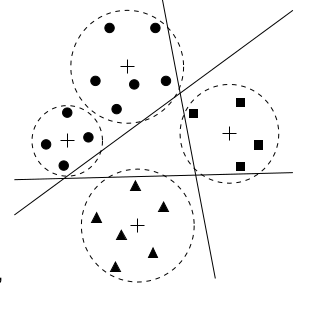
\includegraphics[width=0.4\textwidth]{img/RBF/MLPvsRBF.png}
    \caption{Klassifikation: MLP mit Hyperebenen vs. RBF mit Hyperkugeln}
    \label{ch_RBF_MLPvsRBF}
\end{figure}


\chapter{Methoden zur Merkmalsreduktion}
\paragraph{Ziele}
\begin{itemize}
    \item kompetitive Netze führen eine Reduktion der Datenpunkte auf einige Prototypen durch 
    \item Kohohnen SOM: Reduktion der Datenpunkte auf Prototypen und Visualisierung der Prototypen durch nachbarschaftserhaltende Projektion 
    \item es wird versucht eine Reduktion der Datenpunkte auf repräsentative Merkmale zu erhalten, welche sich durch lineare Kombination der vorhandenen Merkmale ergeben
\end{itemize}

\section{Hauptachsentransformation}
\subsection{Hauptachsen}
\begin{itemize}
    \item Merkmale in denen die Daten nicht variieren sind bedeutungslos 
    \item Hauptachsen sind ONS $(v_i)_{i=1}^l\in\mathbb{R}^d$ mit $l\leq d$, dass die Ursprüglichen Daten mit möglichst geringen Fehler repräsentiert
    \item 1. Hauptachse beschreibt Vektor $v_1$ mit der größten Variation\\
        2. Hauptachse beschreibt Vektor $v_2$ mit zweitgrößter Variation und senkrecht auf $v_1$\\
        und so weiter
\end{itemize}

\subsection{Hauptachsentransformation}
\begin{itemize}
    \item Gegeben sei eine Datenmenge mit $M$ Punkten $x^\mu\in\mathbb{R}^d$ als Datenmatrix $X\in\mathbb{R}^{M\times d}$
    \item Die einzelnen Merkmale (Spaltenvektoren in X) haben Mittelwert 0
    \item Die Projektion zweier Vektoren $v\in\mathbb{R}^d$ auf $x \in X$ ist gegeben durch $\langle v,x^\mu \rangle = \sum_{i=1}^dv_ix_i^\mu $
    \item Für alle Datenpunkte ixt $Xv$ der Vektor mit den Datenprojektionen
    \item $(v_i)_{i=1}^d\in\mathbb{R}^d$ ein ONS
    \item $l<d$. Für $x\in\mathbb{R}^d$ gilt dann mit $\alpha_i = \langle x,v_i \rangle$\\ 
        $x = \alpha_1v_1 + \dots + \alpha_lv_l + \dots +\alpha_dv_d$\\
        Definiere $\Tilde{x} = \alpha_1v_1 + \dots + \alpha_lv_l$
\end{itemize}

Es wird nun der Fehler zwischen $x$ und $\Tilde{x}$ betrachtet.
\begin{equation*}
    e_l(x)=\norm{x-\Tilde{x}}_2^2 = \norm{\sum_{j=+1}^d\alpha_jv_j}_2^2
\end{equation*}
Es soll nun die Summe des Fehlers über alle Daten minimiert werden
\begin{equation*}
    \sum_\mu e_l(x^\mu) = \sum_\mu \langle \sum_{j=l+1}^d\alpha_j^\mu v_j, \sum_{j=l+1}^d\alpha_j^\mu v_j \rangle = \sum_\mu \sum_{j=l+1}^d(\alpha_j^\mu)^2 \rightarrow \texttt{min}
\end{equation*}

Aus dem oben beschrieben folgt dann
\begin{equation*}
    (\alpha_j^\mu)^2 = \alpha_j^\mu \cdot \alpha_j^\mu = (v_j^Tx^\mu)((x^\mu)^Tv_j) = v_j^T(x^\mu(x^\mu)^T)v_j
\end{equation*}
Mitteln über alle Muster
\begin{equation*}
    \frac{1}{M}\sum_\mu\sum_{j=l+1}^dv_j^T(x^\mu(x^\mu)^T)v_j = \sum_{j=l+1}^dv_j^T\frac{1}{M}\sum_\mu(x^\mu(x^\mu)^T)v_j
\end{equation*}

Durch $R=\frac{1}{M}\sum_\mu(x^\mu(x^\mu)^T)$ ist der Korrelationsmatrix der Datenmenge $X$ gegeben.\\
Es muss also der folgende Term minimiert werden
\begin{equation*}
    \sum_{j=l+1}^dv_j^TRv_j \rightarrow \texttt{min}
\end{equation*}

Damit die $v_j$ nicht zu 0 minimiert werden, muss eine Nebenbedingung eingeführt werden. Wähle $v_j^Tv_j = \norm{v_j}^2$ als Nebenbedingung.\\
Auf dieses Problem kann die Methode der Lagrange Multiplikatoren angewendet werden.
\begin{equation*}
    \varphi(v_{l+1},\dots,v_d) = \sum_{j=l+1}^dv_j^TRv_j - \sum_{j=l+1}^d\lambda_j(v_j^Tv_j-1)
\end{equation*}
hierbei sind $\lambda_j\in\mathbb{R}$ die Lagrange-Multiplikatoren.\\
Differenzieren der Lagrange-Funktion nach $v_j$ liefert dann 
\begin{equation*}
    \frac{\partial\varphi}{\partial v_j} = 2Rv_j-2\lambda_j v_j=0
\end{equation*}
Man erhält daraus das Eigenwertproblem
\begin{equation*}
    Rv_j = \lambda_jv_j \quad j=l+1,\dots,d
\end{equation*}
Das gesuchte ONS $(v_j)_{j=1}^d$ sind also Eigenvektoren von $R$. R ist symmetrisch und nichtnegativ-definit, d.h. alle Eigenwerte sind reell und nichtnegativ.

\paragraph{Vorgehen}
\begin{itemize}
    \item Merkmale auf Mittelwert $\mu=0$ transformieren
    \item Kovarianzmatrix $C=X^TX$ berechnen
    \item Eigenwerte $\lambda_1,\dots,\lambda_d$ und Eigenvektoren $v_1,\dots,v_d$ von C bestimmen
    \item Daten X auf die $d'\leq d$ Hauptachsen projizieren, d.h. $X' = XV$ mit $V=(v_1,v_2,\dots,v_{d'})$
\end{itemize}

Man hat nun also die neue Datenmatrix $X'$ mit M Zeilen und $d'$ Merkmalen erhalten.

\section{Neuronale Hauptachsentransformation}
\subsection{Oja-Lernregel}
\begin{itemize}
    \item Lineare Verrechnung der Eingabe $x$ und dem Gewichtsvektor $c$ (einzelnes lineares Neuron)\\
        $y = \langle x,c \rangle = \sum_{i=1}^nx_ic_i$
    \item Lernregeln von Oja\\
        $\Delta c = l_ty(x-yc)$
    \item Gewichtsvektor $c$ konvergiert gegen die 1. Hauptachse $v_1$ (wenn gilt $l_t\to 0$ bei $t\to\infty$ und $\sum_t l_t = \infty$ und $\sum_t l_t^2<\infty$)    
\end{itemize}

\noindent Hat man die erste Hauptachse erhalten, kann man mit dieser Information die anderen ausrechnen.

\subsection{Sanger-Lernregel}
\begin{itemize}
    \item Verallgemeinerung auf $d'\leq d$ lineare Neuronen mit $d'$ Gewichtsvektoren $c_j$. Die Ausgabe des j-ten Neurons ist gegeben durch\\
    $y_j = \langle x,c_j \rangle$
    \item Lernregel nach Sange\\
        $\Delta c_{ij} = l_ty_j(x_i -\sum_{k=1}^jy_kc_{ik}$
    \item $c_l$ konvergiert gegen die Hauptachsen $v_l$ (wenn Bedingungen von oben gegeben sind)    
\end{itemize}

\end{document}
